\chapter {MOTION SYNTHESIS FRAMEWORK}
\label{chap:msf}
\nomenclature[z57]{\boa}{Basin of Attraction}
\graphicspath{{CombineFramework/CombineFrameworkFigs/EPS/}{CombineFramework/CombineFrameworkFigs/}}
The principal ideas of \moit are discussed in previous two chapters.
The stability of motion is controlled by maintaining the topology.
For the periodic motions, neural oscillator can be used to enhance the structural stability.
And group Transformation provides a mechanism to modify motion with precision.


Questions arise when these ideas are being applied  to \cms.
The first question comes from combining the controller of neural oscillator and symmetry controller.
We must ensure that the combination will violate neither the symmetry nor the topology,
This question is discussed in details in Section~\ref{sec:combin}.


Section~\ref{sec:procframe} provides more detailed information of the pipeline, or the procedure of applying this idea in \cms applications.

%Previous chapters only focus on how to maintain motion primitives, a further question is how motion primitives are connected, for example, how a character transit from walking to running. 
%Section~\ref{sec:manyprimitive} shows how the method for maintaining motion primitive are used for motion primitive transition.
%
%
%
%
%The ideas of Global Motor Invariant and Local Motor Invariant are discussed separately in Chapter~\ref{chap:gi} and Chapter~\ref{chap:li}.
%This chapter focuses on put these ideas into \cms application.
%Two problems arised from combinations in application
%\begin{itemize}
%	\item Combine global and local motor invariant controller together.
%	\item Combine different motion primitives together.
%\end{itemize}

\section{Combined Invariant Control}
\label{sec:combin}
\subsection{ Combine Invariant Control}

Neural control $\uout$ maintains the topology, and local control $ulocal$  maintains the symmetry.
Combining two controllers will violate nor the global or local invariant.

In order to adjust the combined controller for practical applications,
\cpg is applied first to maintain the topology against the structural perturbation. 
Then symmetry controllers are applied to meet application specific constraints.
This idea is illustrated in the following Figure ~\ref{fig:sysoverview}

\begin{figure}[!htbp]
  \begin{center}
      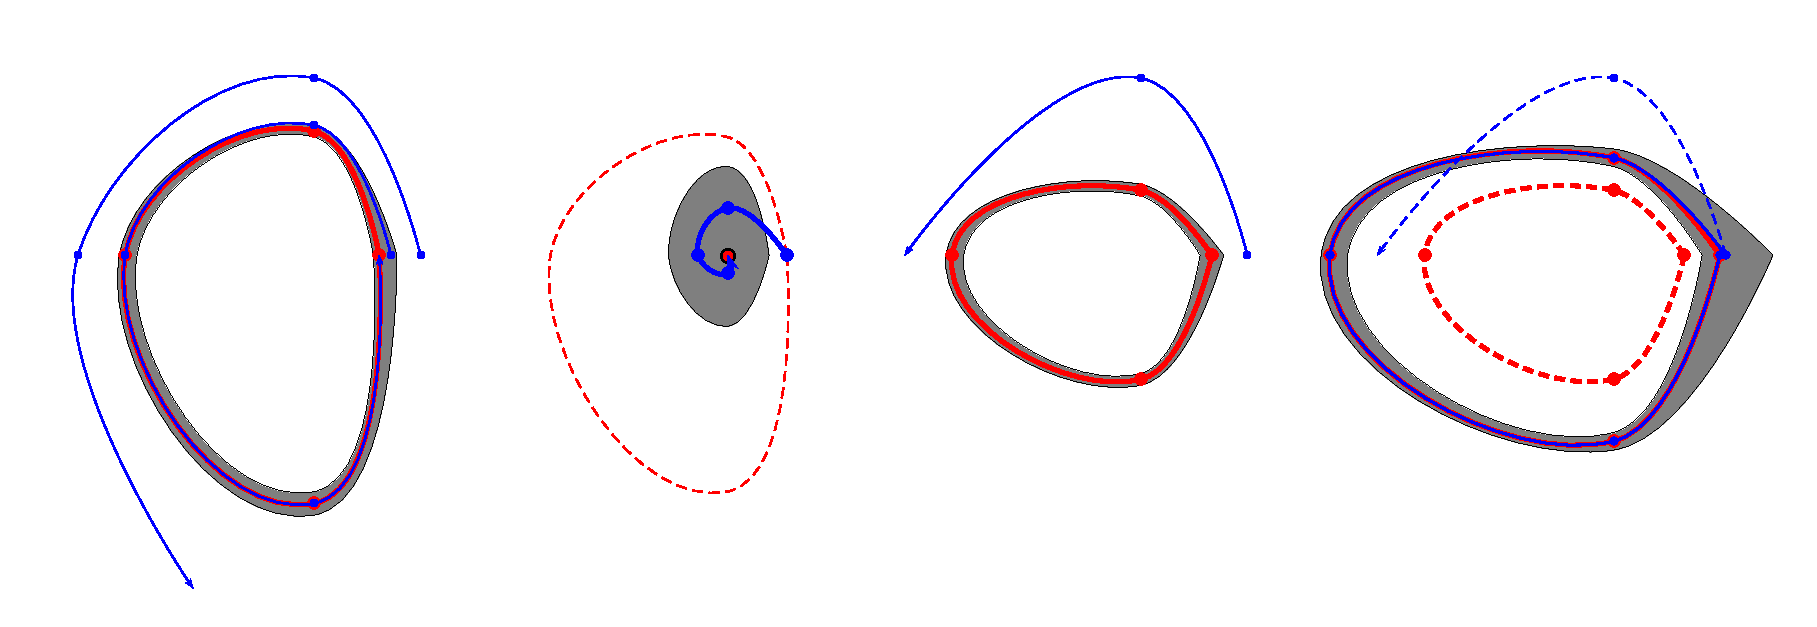
\includegraphics[width=0.7\textwidth]{LimitCircle}
    \caption{System Overview }
    \label{fig:sysoverview}
  \end{center}
\end{figure}





From the perspective in Chapter~\ref{chap:gi},
The inclusion of symmetry control must not violate the topology. 
It is easy to prove that controlled symmetry maintains the topology.
For the controlled symmetry's effect on topology, we have the following theorem:

\begin{mythe}
Transformation of Control Symmetry is Topological Conjugation
\end{mythe}


From the perspective in Chapter~\ref{chap:li},
we must ensure the inclusion of neural oscillator control $\ulocal$ will not break the controlled symmetry.


For this, the parameters of \cpg need to be modified accordingly to maintain the symmetry property.
This is called \emph{Adjoint Transformation}.









\subsection{Adjoint Transformation of \cpg}
\emph{Adjoint Transformation} modifies the parameters of neural oscillator to maintain the symmetry.

For a dynamic system 
\[
\dot{\state}=F(\state)
\]
when controlled by neural oscillator, it becomes 
\begin{equation}
\label{eq:gc}
\dot{\state}=F(\state)+D\uout
\end{equation}
where $D$ is the connection matrix, which describes how the neural oscillator is connected to mechanical system.


When group action $g$ is applied, Equations~\ref{eq:gc} is transformed into
\begin{equation}
\label{eq:cc}
Tg(\dot{\state})=F(g(\state))+DTg(\uout)
\end{equation}




If symmetry is preserved, the Equation~\ref{eq:con} and Equation~\ref{eq:cc} should be equivalent.
\begin{equation}
\label{eq:con}
\dot{\state}=F(\state)+\ulocal+D\tilde{\uout}
\end{equation}
where $\tilde{\uout}$ is the output of neural system after adjoint transformation.

As shown in Equation~\ref{eq:simplematsuta}, since $\uout$ is a complex function of $\uin$,
it is difficult   and not computational efficient to develop a closed form formula.
As an alternative, the idea is to utilize the symmetry property  of Matsuoka Oscillator.
In this way, CPG can be transformed by modifying the parameters.
The transformation scheme is based on the following proposition.


\begin{myprop}
By modifying parameter $\tau_{1,2}$
\[
\tau_{1,2} \mapsto \ep \tau_{1,2}
\]
is equivalent to time scaling of the neural oscillator by parameter $\ep$.
\end{myprop}

This proposition can be easily proved by  substituting $\tilde{\tau}_{1,2}=\ep \tau_{1,2}$, and $\tilde{t}=\frac{t}{\ep}$ into the Matsuoka Oscillator( Equation~\ref{eq:matsuta}), the equation will remain the same.
Based on above the proposition, a scheme of the adjoint transformation is proposed that modifies the parameters $\tau_{1,2}$,$\hin$,$\hout$ and maintains the symmetry of the  coupled system.
The input and output of neural are chosen to maintain the shape.
\begin{enumerate}
\item Modify $\tau$ by the time scaling parameter $\tau \mapsto \ep \tau$.
\item the input variable $w$ and input efficient $\hin$ are modified to make sure the input function satisfy the time scaling symmetry $\uin(t) \mapsto \uin(\frac{t}{\ep})$
\item  Parameters of $\hout$ are modified according to the connection matrix $D$, or how the mechanical system is driven.
If $\uout$ drives the position variable $q$ then, $\hout$ should be multiplied by the position scale factor. 
If $\uout$ drives the velocity,$\hout$ should be  multiplied by the speed scale factor.
If the $hout$ is force and acting on the acceleration $\ddot{q}$, then $\hout$ should be multiplied by the acceleration scale factor.
\end{enumerate}


According to this adjoint transformation strategy, we can get the following theorem
\begin{mythe}
For a transformation group $G$, if the parameters of the neural oscillator are modified according to the adjoint transformation,
combined system preserves symmetry $I^G$.
\end{mythe}
To prove it, readers can check the symmetry by substituting transformed variables into the original system to check the symmetry.
With such a treatment, both the Local Motor Invariant and Global Motor Invariant are maintained
For the specific symmetry types proposed in Chapter~\ref{chap:li},several examples of adjoint transformations are provided


\subsubsection*{ Offset Symmetry.}
For offset symmetry:
\[
(t,q,\qd) \mapsto (t,q+\ep,\qd)
\]
there is no time scaling effect.
To maintain the symmetry,  the simplest way is to select $\uin$ and $\uout$ from the functions in the invariant space$I^G$.
For example, when all  $q$ is transformed by a constant, the difference and the velocity will not be transformed. 
Thus,the input of the neural oscillator is chosen to be the angle difference between the joints or velocity.



\subsubsection*{Time Scaling}
For time scaling:
\[
(t,q,\qd) \mapsto (\frac{t}{\ep},q,\ep \qd)
\]
Adjoint Transformation
$\tau \mapsto \ep \tau $.
The input coefficient $\hin$ and output coefficient $\hout$ are scaled accordingly.
if the output$\uout$ is applied as a force, then it should be scaled by the acceleration factor
\[
 \hout \mapsto \ep^2 \hout
\]
\subsubsection*{ Energy Scaling}
Energy Scaling is a combined action of time scaling and posture scaling:
\[
(t,q,\qd ) \mapsto ( \frac{f(\ep)}{\ep}t ,f(\ep)q,\ep\qd)
\]
the time scaling factor is $\frac{\ep}{f(\ep)}$, 

The parameters $\tau_{1,2}$ are transformed
\[
\tau_{1,2} \mapsto \frac{\ep}{f(\ep)} \tau_{1,2}
\]

The input coefficient is scaled to make the amplitude of the input signal maintained.
\[
\hin \mapsto \frac{\hin}{\ep}
\]

The output coefficient is scaled according to the connection of the control, 
if the output drive the velocity, then the output is $\hout$
\[
\hout \mapsto \ep \hout
\]




\subsection{Example: Height Control of Bouncing Ball}

The Bouncing Ball has the energy scaling symmetry, and a limit cycle emerged when coupled with a neural oscillator.
By combining both motor invariant controllers, stability is maintained and motion can be adjusted precisely. 
When energy transformation is applied to the limit cycle, the bouncing height can be adjusted according to the purpose.

\subsubsection*{Adjoint Transformation}
Supposing the coupled system is bouncing at height of $5$
For the energy scaling:
\[
(t,q,\qd ) \mapsto ( \ep t ,\ep^2 q,\ep \qd)
\]
the time scaling factor is $\ep$, and we have:
\[
\tau_{1,2} \mapsto \ep \tau_{1,2}
\]

The input to the neural oscillator is $\qd$,
\[
\hin \mapsto \frac{\hin}{\ep}
\]
 
Neural Oscillator drives the position of the paddle, the output $\uout$ needs to be scaled by the position scale value.
For $q \mapsto \ep^2q$, we have
\[
 \hout \mapsto \ep^2 \hout
\]

When $\ep^2=3$,  the ball will bounce at height of $15$, and it maintains its topological structure, which is a limit cycle, as shown in Figure ~\ref{fig:energy3}. 
With this method, arbitrary bouncing height can be controlled.


\begin{figure}[!htbp]
  \begin{center}
   	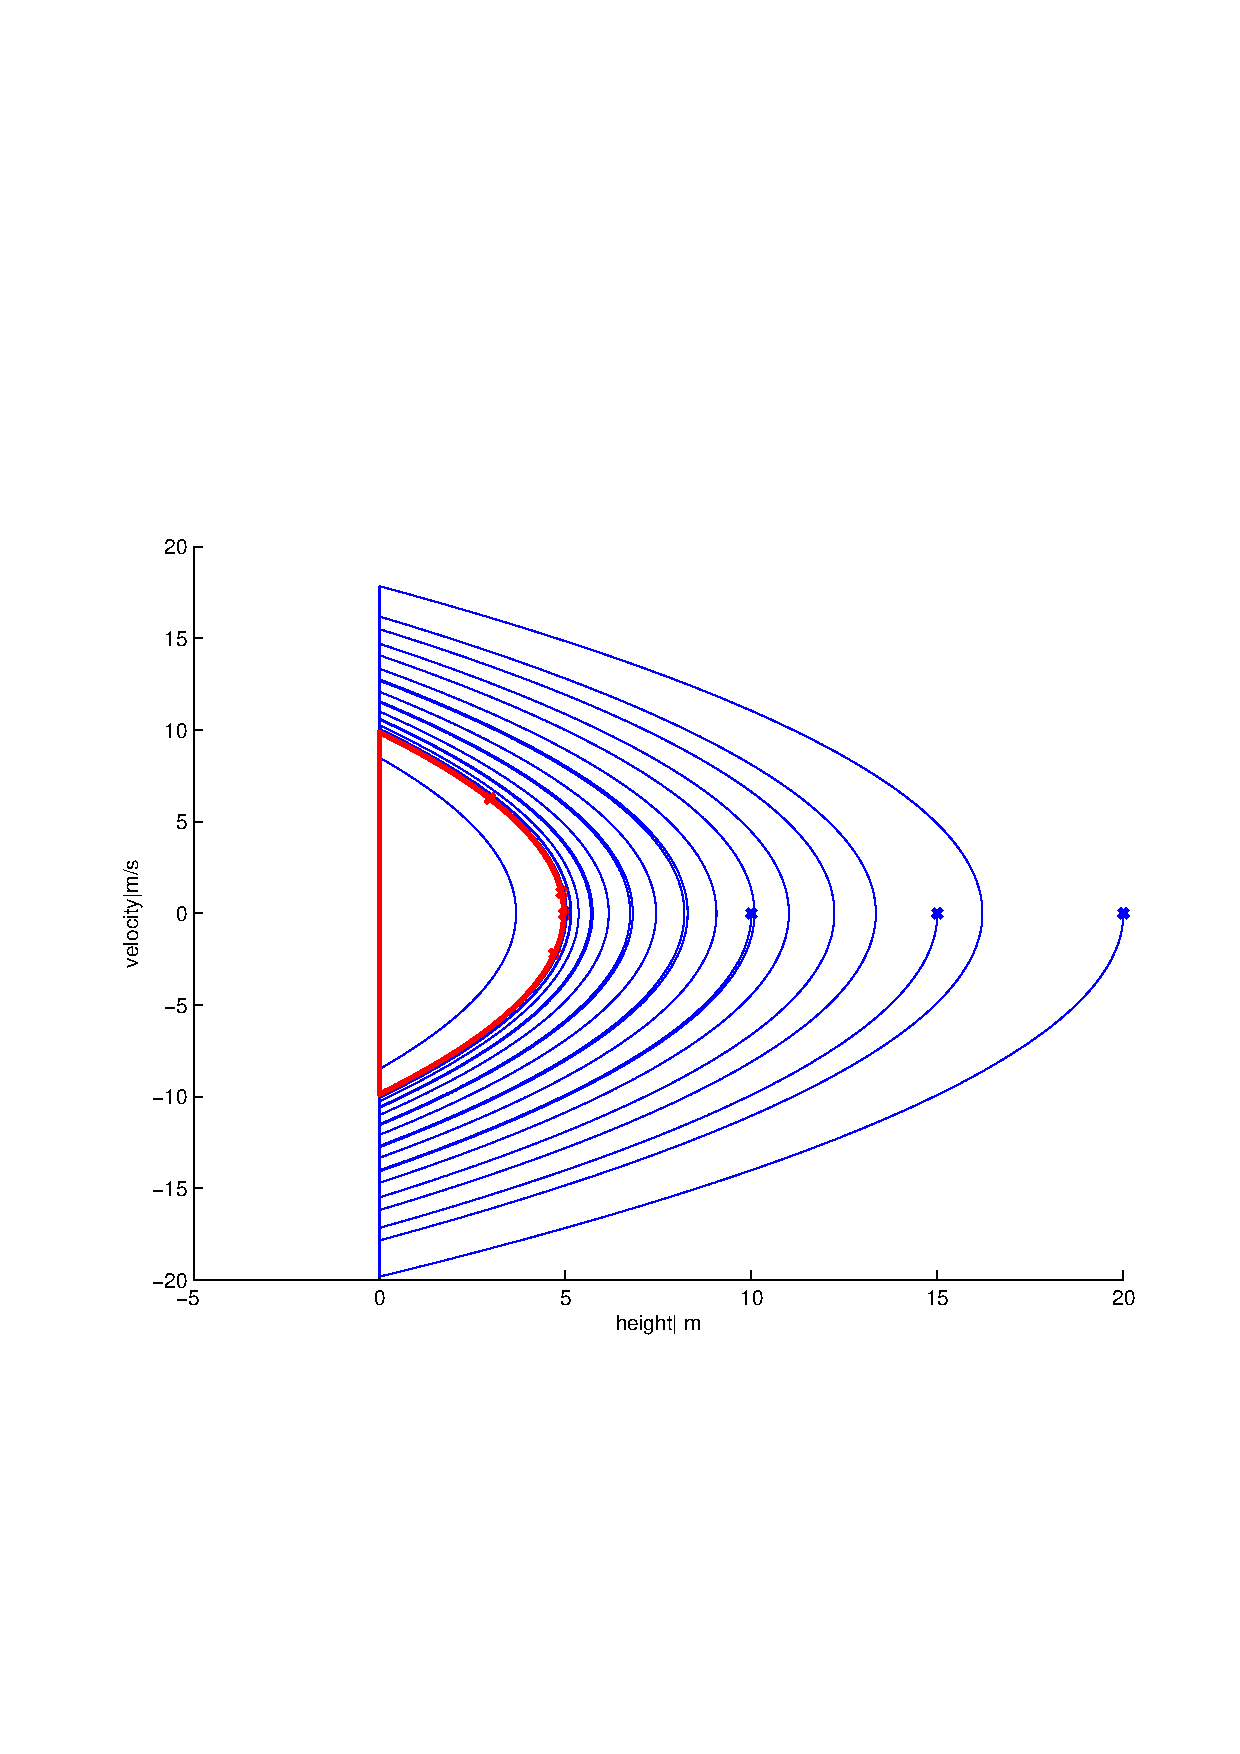
\includegraphics[width=0.7\textwidth]{BouncingBallPhasePlotAction1}
    \caption{Energy Scalling}
    \label{fig:energy1}
  \end{center}
\end{figure} 


\begin{figure}[!htbp]
  \begin{center}
	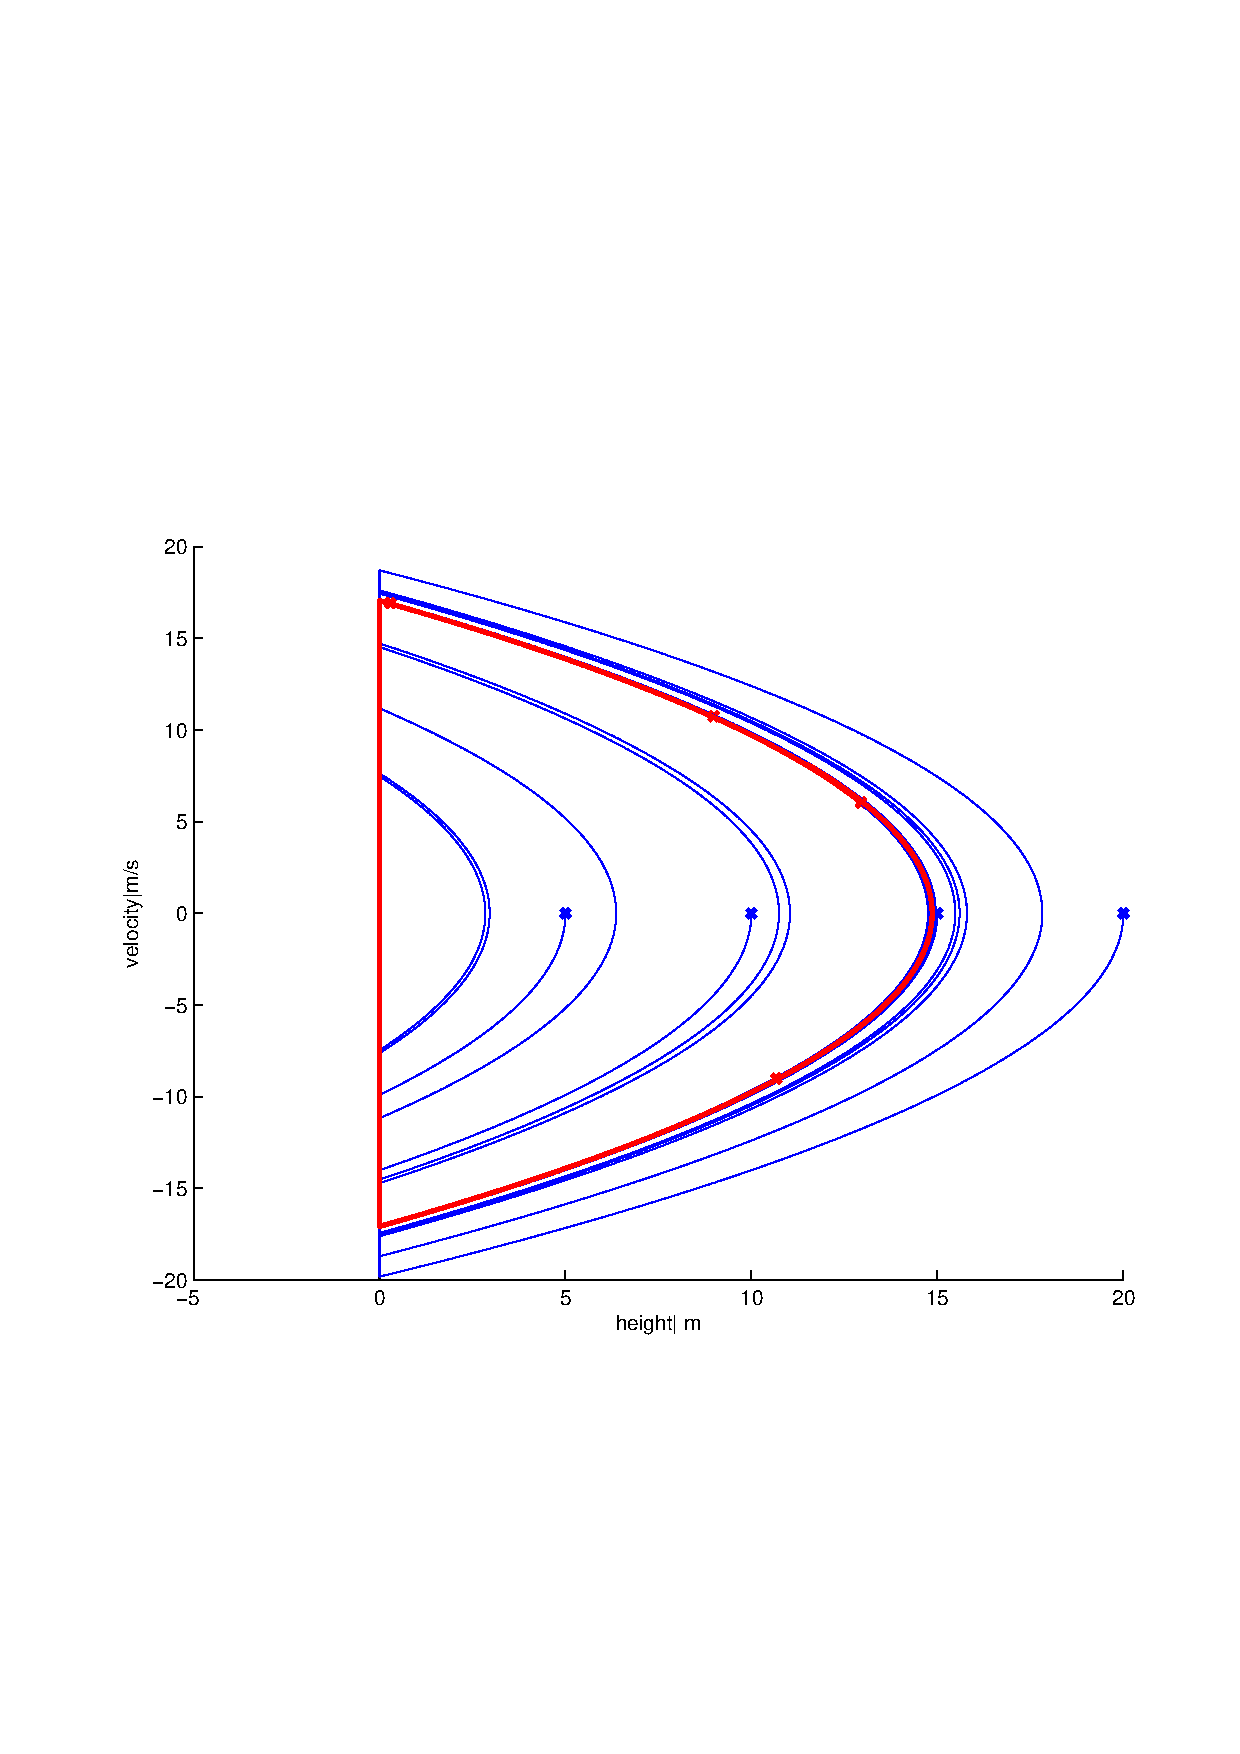
\includegraphics[width=0.7\textwidth]{BouncingBallPhasePlotAction3}
    \caption{Energy Scaling}
    \label{fig:energy3}
  \end{center}
\end{figure}

\section{Combine Motion Primitives}
\label{sec:manyprimitive}

\subsection{Dynamic Motion Graph}
Virtual characters are capable of many types of motions and switch between them fluently.
\emph{Motion Graph}\citep{kovar2008motion} is proposed for data-driven \cms:
basic motion tasks are recorded, and a graph describes how a character can change from one motion into another motion. 
For the transitional motions, the most popular synthesizing method is blending.


\moit implies an idea similar to the motion graph but from a different direction.
Usually, traditional \emph{motion graph}s are manually designed, while \moit proposes an idea which generates the motion graph from the dynamics automatically.
In theory,the topological structure of a dynamic system can be represented by a  graph.
Each motion primitive is represented as a node, and two nodes are connected only if their basins of attraction({\boa}s) are in neighbour.

\begin{figure}[!htbp]
  \begin{center}
	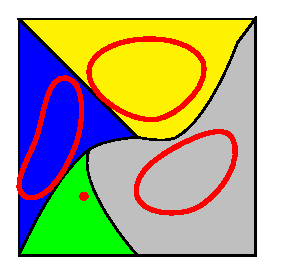
\includegraphics[width=0.7\textwidth]{CellBoa}
    \caption{Phase Plot of Motion Primitives}
    \label{fig:manyprimitives}
  \end{center}
\end{figure}


\begin{figure}[!htbp]
  \begin{center}
      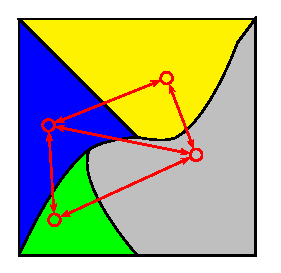
\includegraphics[width=0.7\textwidth]{CellTopology}
    \caption{The Graph Structure of A Dynamic System}
    \label{fig:manyprimitivesgraph}
  \end{center}
\end{figure}

For example, Figure~\ref{fig:manyprimitives} shows the phase portrait of a hypothetical dynamic system.
Its phase space is divided into four regions of different colors.
The four \boa s, within each region, there is a limit cycle(deep coloured).
The graph in Figure~\ref{fig:manyprimitivesgraph} shows the corresponding graph structure, in which each node represents the \boa of the same color in Figure~\ref{fig:manyprimitives}, the connecting edge means the basin of {\boa}s of connected motion primitives are in neighbour, which can also be verified by Figure~\ref{fig:manyprimitives}.


\subsection{Dynamic Motion Transition}

In real life, the transition of motion is an adaptive and interesting phenomenon.
However, Blending techniques tend to generate motions with little variations. 
Blending techniques tend to generate motions with little variation.
While based on the control method for maintaining motion primitives, MoIT proposes a physics based method for generation of transitional motion.



\begin{figure}[!htbp]
  \begin{center}
      \includegraphics[width=0.7\textwidth]{MotionPrimitiveTransition}
    \caption{Motion Primitive Transition}
    \label{fig:motion-transition}
  \end{center}
\end{figure}

From the geometrical perspective, motion transition means putting the current $\state$ out of one \boa into another.
This process is illustrated in Figure~\ref{fig:motion-transition} where the current state represented by the black dot lies in the left region of \boa and will converge to the red limit cycle over time.

The neighbouring region is the \boa of another primitive, in which if the current state lies, will converge to the green limit cycle.
Because two basins of attractions do not overlap, the transition will not happen automatically without effort. 
From a geometrical viewport,  to make motion transition happens, a small action is needed to push the state across the boundary, represented by the red line. This can be achieved by many efficient methods.


\subsubsection*{Entrainment Overlap}
Empirically,when a \cpg is applied for one motor primitive $\mathcal{A}$, the basin of attraction $\BOA{A}$ is enlarged.
Supposing the enlarged basin of attraction  is  represented by $\BOA{A'}$,
if \cpg are applied for two motion primitives $\mathcal{A_1,A_2}$ in neighbour, the enlarged basins of attraction ($\BOA{A_1'}$ and $\BOA{A_2'}$ ) will overlap. 
\[
O =
\BOA{A_1'} 
\bigcap \BOA{A_2'} 
\neq \varnothing
\]
where $O$ is the overlapping region.

\begin{figure}[!htbp]
  \begin{center}
      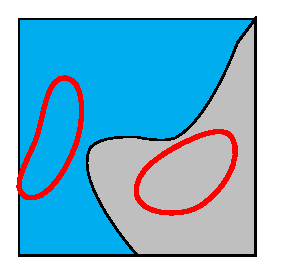
\includegraphics[width=0.7\textwidth]{CPGOVERLAY}
    \caption{ Motion Transition based on Motion Primitives Overlap}
    \label{fig:motion-overlay}
  \end{center}
\end{figure}
 
If  state $\state$ lies in the $O$, the dynamic system will converge to a different attractor by switching the \cpg controller.
Figure~\ref{fig:motion-overlay} shows the idea through an example.
The phase plot shown two motion primitives which are connected.
Basins of attraction of natural dynamics are represented by the dot line, which do not overlap.
When \cpg is applied, two basins of attraction are enlarged, and the shared region is coloured in pink color.
When the current state lies in $O$, the state will converge to the left limit cycle if the \cpg of the left region is activated  and converge to the right limit cycle if the right \cpg is activated.
Motion Primitive can be switched in this manner.






\subsubsection*{Transform Method}
Controlled Symmetry can also be applied for motion primitive transition.
We can change the \boa where the current state lies by transforming the phase portrait.

\begin{figure}[!htbp]
  \begin{center}
      \includegraphics[width=0.7\textwidth]{TransformOverlay}
    \caption{Offset Transition}
    \label{fig:transform-offset}
  \end{center}
\end{figure}




As shown in Figure~\ref{fig:transform-offset}, the phase portrait of natural dynamic system is the same as that of Figure~\ref{fig:motion-overlay}, which is also indicated by the dot.
The current state converges to the left (red) limit cycle.
By applying offset action to the dynamic system, the phase portrait  moves leftward, which makes current state lie in the right \boa.
Over time, current state will converge to the right(green) limit cycle,  motion primitive is changed accordingly.







\subsection{Combined Method}
Both methods utilize the natural dynamics and  result in a physically realistic transition.
However, both methods require x lies in the overlapping region.
In the motor invariant theory, the current state x is not directly controlled. The measure is to make the overlap region O cover part of both attractors.

As shown in Figure~\ref{fig:Combine}.
The overlap region covers both attractors $\mathcal{A}$, $\mathcal{A'}$, bidirectional transitions are possible when motion converge to to the limit cycle.

More importantly, when transformation is applied, the action is applied to the dynamic system. Thus both motion primitives are transformed, called the the \emph{connection transformation }. 
As shown in Figure~\ref{fig:Combine}, both motion primitives are transformed by the time scaling action.

\begin{figure}[!htbp]
  \begin{center}
      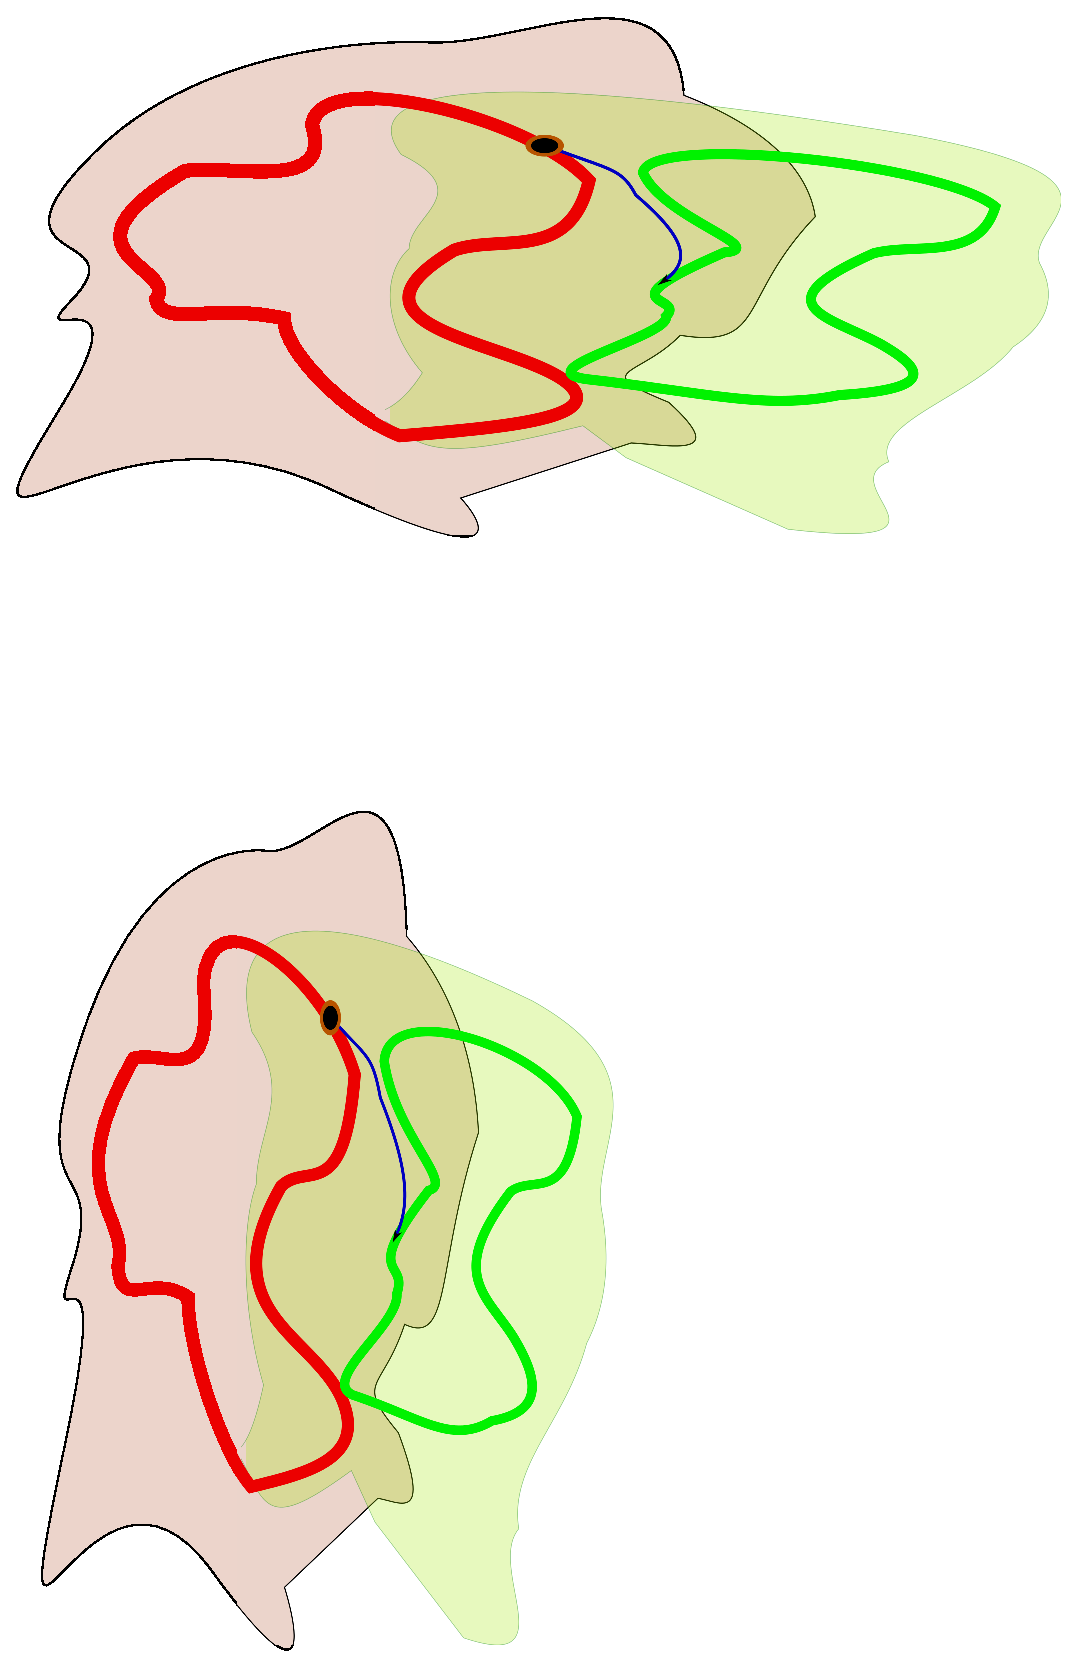
\includegraphics[width=0.7\textwidth]{ConbineMethod}
    \caption{Combined Method}
    \label{fig:Combine}
  \end{center}
\end{figure}

\section{Motion Synthesis Framework}
\label{sec:procframe}
While this procedure may appear mathematically complex, applying this method for motion synthesis is straightforward. 
You will need:
\begin{enumerate}
\item a mechanical oscillator $F(\x)$ which best describes the body and environment
\item a neural oscillator (for example, the Matsuoka oscillator in Equation~\ref{eq:matsuta}) and associated parameters,that form a limit cycle

\item an action $g \in G$ which adapts the problem to the current environment (we present three possible operators in Section~\ref{sec:groupandsymmetry}). 
The adjoint system transformation  is applied to the neural oscillator parameters.

\item an integrator to solve the system (we use the fourth order Runge--Kutta method provided in the {MATLAB} function \emph{ode45}).
\end{enumerate}
In the following chapters, this method is applied to generating adaptive motions.



